\chapter{Anti-unification ASTs}\label{AUAST}

\RW{New intro blurb needed. Basically, you need to point out how Jigsaw does not suffice, which hopefully you will have demonstrated in the previous chapter.  It's not clear to me why this is separate from the next chapter.  Perhaps combine them?}

Section~\ref{AUAST} describes the development of an anti-unification algorithm for our application.
\RW{Describe testing/evaluation.}

\section{Constructing the AUAST} \label{AUAST}
\RW{This is a concrete implementation, not a generic idea, at least not the way it is described.  I strongly suggest that you give a generic description of your assumptions about ASTs then relate AUASTs to those, then talk about implementation details.}
An anti-unifier AST (AUAST) is an extended form of AST that allows the insertion of variables in place of any node in the tree structure, including both subtrees and leaves, to indicate variations between original structures. The AUAST addresses the limitations of AST to construct an anti-unifier by adding the following structural properties:
\begin{itemize} [leftmargin=.4in]
\item \textit{Simple Variable Property}: an extension of simple property referring to two simple values to allow the insertion of variables in place of leaves.
\end{itemize}
\begin{itemize} [leftmargin=.4in]
\item \textit{Child Variable Property}: an extension of child property referring to two child AST nodes to allow the insertion of variables in place of subtrees.
\end{itemize}
The anti-unification of AUASTs of logging calls in Figures~\ref{ch3-ex1} and~\ref{ch3-ex2} is depicted in Figure~\ref{fig:logging-anti}. The structural variables $X$ and $Y$ are used to abstract away the structural variations.  The substitutions are defined in Equations~\ref{eq:theta1} and~\ref{eq:theta2}.

\begin{align}
\Theta_1 = (X \rightarrow \text{ \textsf{\small WARNING}}, Y \rightarrow \text{ \textit{additionExpression}(}\hspace*{3cm}\nonumber\\
\text{\textit{methodCall}(\textit{simpleName}(\textsf{\small getClassName}), \textit{arguments}()),}\nonumber\\
\text{\textit{stringLiteral}(\textsf{\small "should extend ..."}),}\hspace*{4cm}\nonumber\\
\text{\textit{methodCall}(\textit{simpleName}(\textsf{\small handleMessage}), \textit{arguments}()))})\hspace*{-1em}\label{eq:theta1}
\end{align}

\begin{align}
\Theta_2 = (X \rightarrow \text{ \textsf{\small ERROR}}, Y \rightarrow \text{ \textit{additionExpression}(}\hspace*{3cm}\nonumber\\
\text{\textit{stringLiteral}(\textsf{\small "Unknown action: "})},\nonumber\\
\text{ \textit{simpleName}(\textsf{\small actionName}))})\hspace*{-1cm}\label{eq:theta2}
\end{align}

%\item it can be mapped to our recursive definition of a term, where AST nodes and simple values may be viewed as function-symbols and constants, respectively

\begin{figure}[p]
\begin{small}
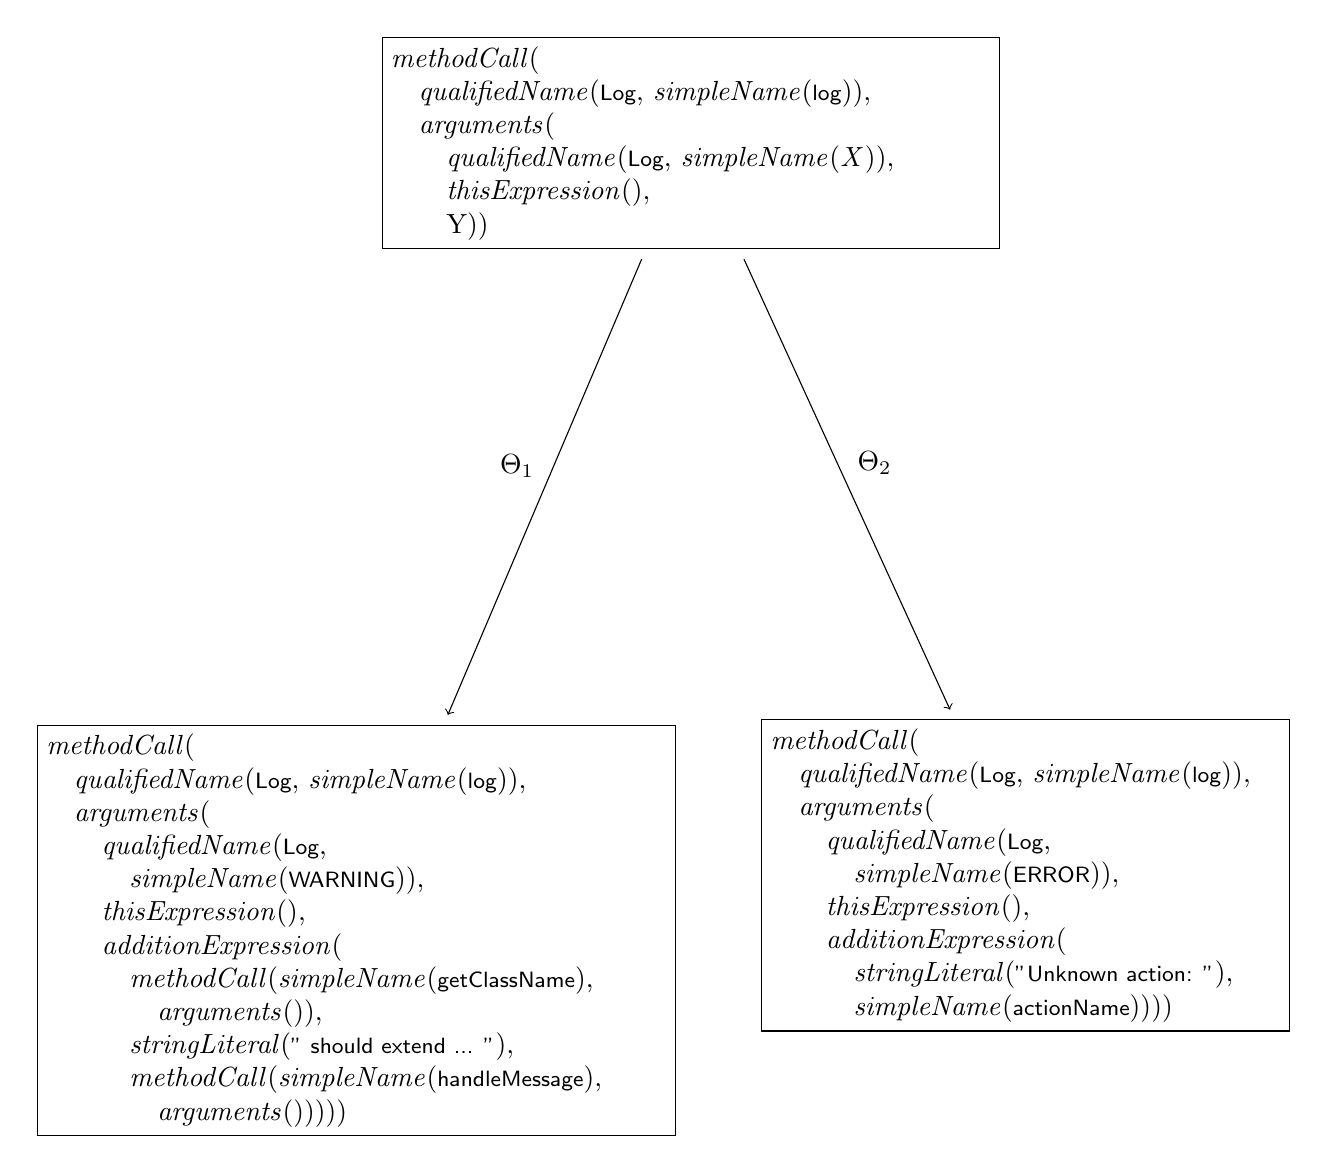
\begin{tikzpicture}
\node(a) at (4.25,10) {%
\fbox{\parbox[b][][b]{3in}{%
\text{\textit{methodCall}(}\\
\text{\hspace*{1em}\textit{qualifiedName}(\textsf{\footnotesize Log}, \textit{simpleName}(\textsf{\footnotesize log})),}\\
\text{\hspace*{1em}\textit{arguments}(}\\
\text{\hspace*{2em}\textit{qualifiedName}(\textsf{\footnotesize Log}, \textit{simpleName}(\textit{X})),}\\
\text{\hspace*{2em}\textit{thisExpression}(),}\\
\text{\hspace*{2em}Y))}}}%
};
\node(b) at (0,0) {%
\fbox{\parbox[t][][b]{3.1in}{%
\text{\textit{methodCall}(}\\
\text{\hspace*{1em}\textit{qualifiedName}(\textsf{\footnotesize Log}, \textit{simpleName}(\textsf{\footnotesize log})),}\\
\text{\hspace*{1em}\textit{arguments}(}\\
\text{\hspace*{2em}\textit{qualifiedName}(\textsf{\footnotesize Log},}\\ \text{\hspace*{3em}\mbox{\textit{simpleName}(\textsf{\footnotesize WARNING})}),}\\
\text{\hspace*{2em}\textit{thisExpression}(),}\\
\text{\hspace*{2em}\textit{additionExpression}(}\\
\text{\hspace*{3em}\textit{methodCall}(\textit{simpleName}(\textsf{\footnotesize getClassName}),}\\ \text{\hspace*{4em}\textit{arguments}()),}\\
\text{\hspace*{3em}\textit{stringLiteral}(\textsf{\footnotesize " should extend ... "}),}\\
\text{\hspace*{3em}\textit{methodCall}(\textit{simpleName}(\textsf{\footnotesize handleMessage}),}\\ \text{\hspace*{4em}\textit{arguments}()))))}}}%
};
\node(c) at (8.5,0.7) {%
\fbox{\parbox[t][][b]{2.55in}{%
\text{\textit{methodCall}(}\\
\text{\hspace*{1em}\textit{qualifiedName}(\textsf{\footnotesize Log}, \textit{simpleName}(\textsf{\footnotesize log})),}\\
\text{\hspace*{1em}\textit{arguments}(}\\
\text{\hspace*{2em}\textit{qualifiedName}(\textsf{\footnotesize Log},}\\ \text{\hspace*{3em}\mbox{\textit{simpleName}(\textsf{\footnotesize ERROR})}),}\\
\text{\hspace*{2em}\textit{thisExpression}(),}\\
\text{\hspace*{2em}\textit{additionExpression}(}\\
\text{\hspace*{3em}\textit{stringLiteral}(\textsf{\footnotesize "Unknown action: "}),}\\
\text{\hspace*{3em}\textit{simpleName}(\textsf{\footnotesize actionName}))))}}}%
};

\draw[->](a) -- (b) node[pos=0.5,above]{$\Theta_1\qquad$};
\draw[->](a) -- (c) node[pos=0.5,above]{$\qquad\Theta_2$};
\end{tikzpicture}
\end{small}
\caption{Anti-unification of the AUASTs of the logging calls in Examples 1 and 2.\label{fig:logging-anti}}
\end{figure}
%The AUASTs of log Method Invocation nodes from the Java classes in Figure~\ref{ch3-ex1} and Figure~\ref{ch3-ex2}.

Applying higher-order anti-unification on AUAST structures could help to construct a structural generalization by maintaining the common pieces and abstracting the differences away using variables. However, it is not comprehensive enough to solve our problem as it does not consider background knowledge about AST structures, such as syntactically different but semantically relevant structures, missing structures, and different ordering of arguments. In the following section, we will look at an extension of anti-unification, higher-order anti-unification modulo theories, and how it can sufficiently address the limitations of anti-unification in our context.


%\begin{align}
%\Theta_1 = (W &\rightarrow \text{ \textsf{\small WARNING}},\nonumber\\
%X &\rightarrow \text{ \textit{methodCall}(\textit{simpleName}(\textsf{\small getClassName}), \textit{arguments}())},\nonumber\\
%Y &\rightarrow \text{ \textsf{\small "should extend EditPlugin not EBPlugin since it has an empty "}},\nonumber\\
%Z &\rightarrow \text{ \textit{methodCall}(\textit{simpleName}(\textsf{\small handleMessage}), \textit{arguments}())})\label{eq:theta1}\\
%\Theta_2 = (W &\rightarrow \text{ \textsf{\small ERROR}},\nonumber\\
%X &\rightarrow \text{ \NIL{}},\nonumber\\
%Y &\rightarrow \text{ \textsf{\small "Unknown action: "}},\nonumber\\
%Z &\rightarrow \text{ \textit{simpleName}(\textsf{\small actionName})})\label{eq:theta2}
%\end{align}
%
%%\item it can be mapped to our recursive definition of a term, where AST nodes and simple values may be viewed as function-symbols and constants, respectively
%
%\begin{figure}[p]
%\begin{small}
%\begin{tikzpicture}
%\node(a) at (4.25,10) {%
%\fbox{\parbox[b][][b]{3in}{%
%\text{\textit{methodCall}(}\\
%\text{\hspace*{1em}\textit{qualifiedName}(\textsf{\footnotesize Log}, \textit{simpleName}(\textsf{\footnotesize log})),}\\
%\text{\hspace*{1em}\textit{arguments}(}\\
%\text{\hspace*{2em}\textit{qualifiedName}(\textsf{\footnotesize Log}, \textit{simpleName}(\textit{W})),}\\
%\text{\hspace*{2em}\textit{thisExpression}(),}\\
%\text{\hspace*{2em}\textit{additionExpression}(\textit{X}, \textit{stringLiteral}(\textit{Y}), \textit{Z})))}}}%
%};
%\node(b) at (0,0) {%
%\fbox{\parbox[t][][b]{3.1in}{%
%\text{\textit{methodCall}(}\\
%\text{\hspace*{1em}\textit{qualifiedName}(\textsf{\footnotesize Log}, \textit{simpleName}(\textsf{\footnotesize log})),}\\
%\text{\hspace*{1em}\textit{arguments}(}\\
%\text{\hspace*{2em}\textit{qualifiedName}(\textsf{\footnotesize Log},}\\ \text{\hspace*{3em}\mbox{\textit{simpleName}(\textsf{\footnotesize WARNING})}),}\\
%\text{\hspace*{2em}\textit{thisExpression}(),}\\
%\text{\hspace*{2em}\textit{additionExpression}(}\\
%\text{\hspace*{3em}\textit{methodCall}(\textit{simpleName}(\textsf{\footnotesize getClassName}),}\\ \text{\hspace*{4em}\textit{arguments}()),}\\
%\text{\hspace*{3em}\textit{stringLiteral}(\textsf{\footnotesize " should extend ... "}),}\\
%\text{\hspace*{3em}\textit{methodCall}(\textit{simpleName}(\textsf{\footnotesize handleMessage}),}\\ \text{\hspace*{4em}\textit{arguments}()))))}}}%
%};
%\node(c) at (8.5,0.7) {%
%\fbox{\parbox[t][][b]{2.55in}{%
%\text{\textit{methodCall}(}\\
%\text{\hspace*{1em}\textit{qualifiedName}(\textsf{\footnotesize Log}, \textit{simpleName}(\textsf{\footnotesize log})),}\\
%\text{\hspace*{1em}\textit{arguments}(}\\
%\text{\hspace*{2em}\textit{qualifiedName}(\textsf{\footnotesize Log},}\\ \text{\hspace*{3em}\mbox{\textit{simpleName}(\textsf{\footnotesize ERROR})}),}\\
%\text{\hspace*{2em}\textit{thisExpression}(),}\\
%\text{\hspace*{2em}\textit{additionExpression}(}\\
%\text{\hspace*{3em}\textit{stringLiteral}(\textsf{\footnotesize "Unknown action: "}),}\\
%\text{\hspace*{3em}\textit{simpleName}(\textsf{\footnotesize actionName}))))}}}%
%};
%
%\draw[->](a) -- (b) node[pos=0.5,above]{$\Theta_1\qquad$};
%\draw[->](a) -- (c) node[pos=0.5,above]{$\qquad\Theta_2$};
%\end{tikzpicture}
%\end{small}
%\caption{The anti-unification of the AUASTs of the logging calls in Examples 1 and 2.\label{fig:logging-anti}}
%\end{figure}
%%The AUASTs of log Method Invocation nodes from the Java classes in Figure~\ref{ch3-ex1} and Figure~\ref{ch3-ex2}.

%Applying higher-order anti-unification on AUAST structures could help to construct a structural generalization by maintaining the common pieces and abstracting the differences away using variables. However, it is not comprehensive enough to solve our problem as it does not consider background knowledge about AST structures, such as syntactically different but semantically relevant structures, missing structures, and different ordering of arguments. In the following section, we will look at an extension of anti-unification, higher-order anti-unification modulo theories, and how it can sufficiently address the limitations of anti-unification in our context.



\begin{figure} [H]
  \centering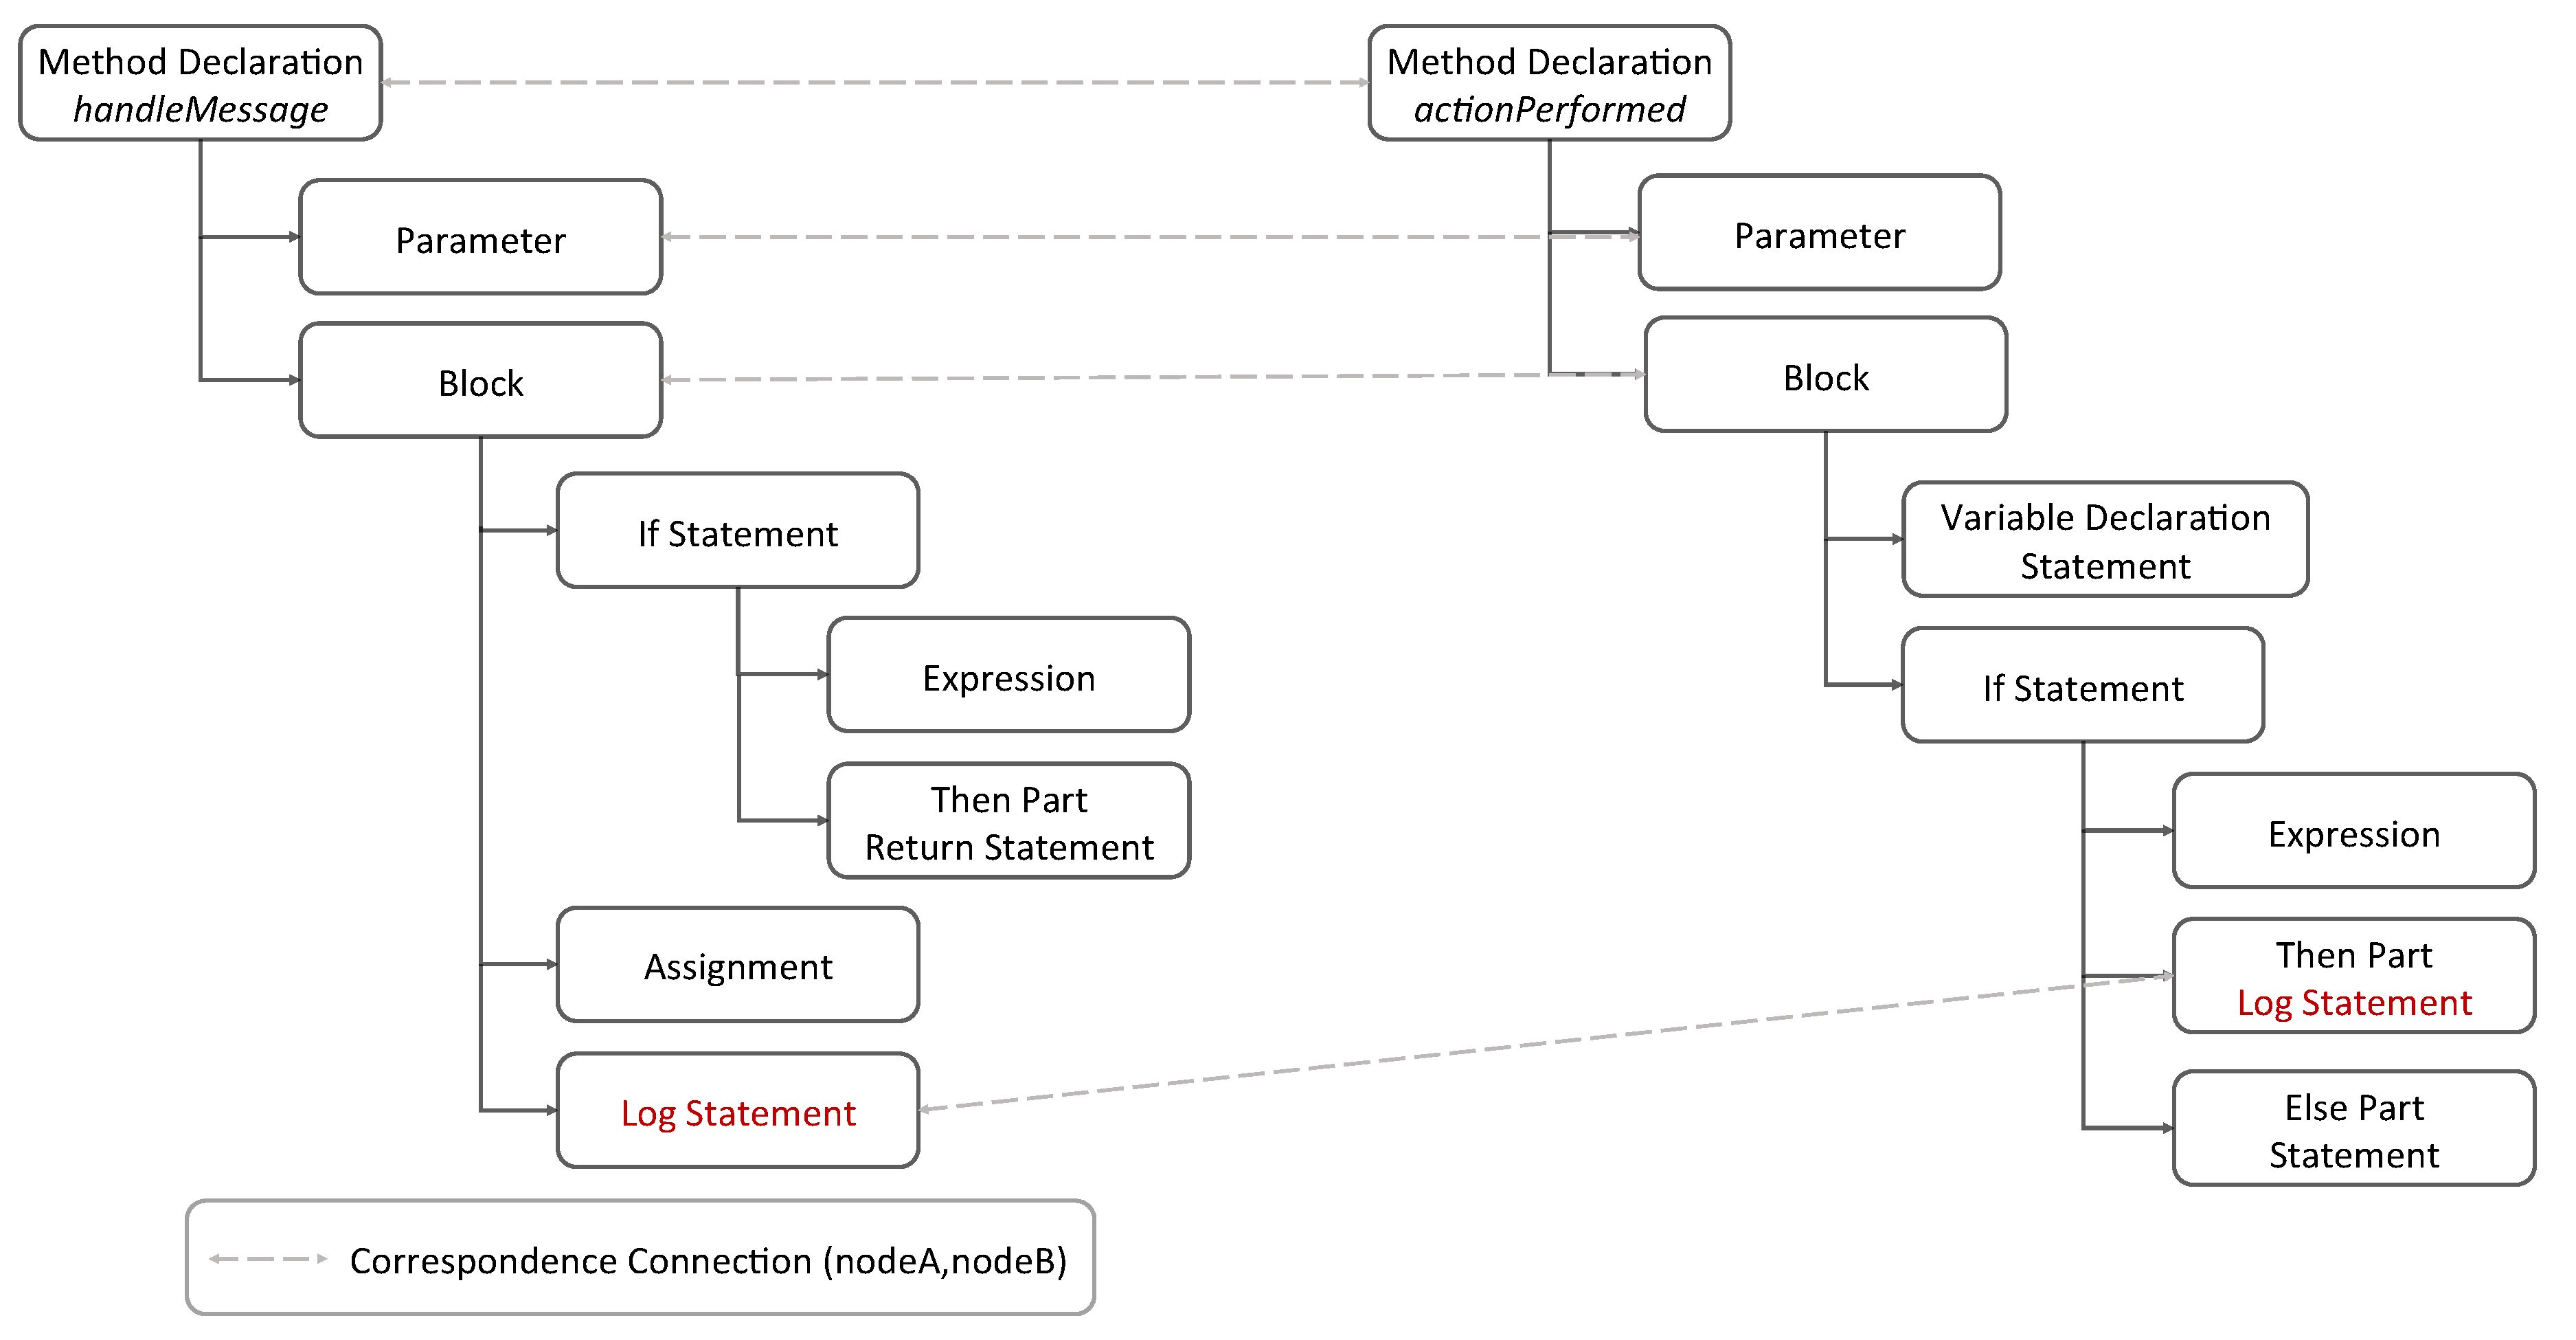
\includegraphics [width = \textwidth]{Drawing4/FirstCorr.pdf}
  \caption{Simple CAST structure of examples in Figures~\ref{ch3-ex1} and~\ref{ch3-ex2}. The links between AST nodes indicate structural correspondence connections created by the Jigsaw framework along with the similarity value.}
  \label{fig:meth-ast-1}
\end{figure}

However, the Jigsaw tool does not suffice to construct an anti-unifier that is the best fit to our application. In addition, the Jigsaw similarity function does not measure the similarity of two logged Java classes with a focus on logging calls, which is needed in our context. To address these issues, we should develop a greedy selection algorithm to approximate the best anti-unifier by determining the best correspondence for each node. In the following chapter, we will discuss our approach to construct structural generalizations and our implementation by means of the higher-order anti-unification modulo theories and the Jigsaw framework.

\section{Evaluation}
\RW{TBD}

\section{Summary}  \label{summary}
In this chapter, we described anti-unification as a technique to construct a common generalization of two given terms. We have also introduced an extended form of anti-unification, which is called higher-order anti-unification modulo theories, where a set of equivalence equations can be applied on higher-order extended structures to incorporate background knowledge. In addition,
we provided a brief description of AST that maps Java source code in a tree structure form, and why an extended form of it, named AUAST, is required to create higher-order structures specific to our problem context. Finally, we discuss the Jigsaw framework and how it could assist us in determining the potential structural correspondences.
